\documentclass{article}
  % M�rgenes
  \textheight    = 20cm
  \textwidth     = 18cm
  \topmargin     = -2cm
  \oddsidemargin = -1cm
  % Sangr�a
  \parindent     =  0mm
  %Paquetes 
  %  deben venir con la distribuci�n TeX 
  %  o se pueden poner en la misma carpeta de este archivo .tex
  \usepackage{amsmath, amssymb, amsfonts, latexsym}
  \usepackage[T1]{fontenc}
  \usepackage[latin1]{inputenc}
  \usepackage{graphicx}
  \usepackage{pstricks}
  \title{Diseinua}
  \author{Ieltzu Irazu, Mikel de Velasco, Jorge Nieto}
  \date{29 de enero de 2010}

  %Inicio del cuerpo del documento
\begin{document}
\newpage
\maketitle
\begin{center}
	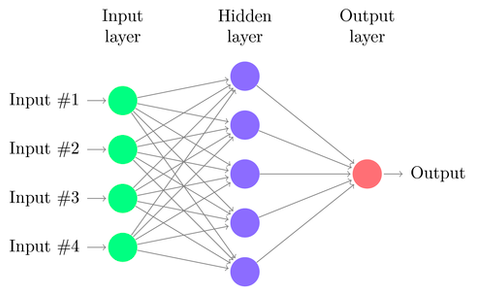
\includegraphics[width=10cm]{img/portada.png} 
\end{center}
\newpage
\section{Azaleko Orria / Aurkibidea}
\begin{enumerate}
	\item {\sc Azaleko Orria / Aurkibidea\dotfill 2}
	\item {\sc Aurkezpena\dotfill 3}
	\item {\sc Klaseen diseinua\dotfill 3}
\end{enumerate}
\newpage
\section{Aurkezpena}
Dokumentu honen bidez, 	
Multilayer Perceptron eta Naive Bayes eredu igarleak konparatzen ditu.
\section{Klaseen diseinua}
Proiektua hiru atal nagusitan banandu dugu. Lehenengoan, datuak aurreprozezatzen dira, bigarrenean, eredua aterako da eta azkenik instantzia berriak ebaluatzeko jarriko dugu.
\begin{enumerate}
	\item \textbf{Aurreprozezamendua} \\
		Atal honetan, bereiziki ``R-weka.filters.unsupervised.attribute.Obfuscate'' relation-a duten arff fitxategiekin (praktika honetan lan egin behar zirenak) lan egingo dugu. Horregatik behean aipatzen diren filtroak praktika honekin lan egiteko daude. \\
		Aurre prozezamenduan horrengo klase eta metodoak erabiliko ditugu.
		\begin{enumerate}
			\item {\bf Aurreprozezamendua:}\\
			Klase hau, {\red aurreprozezamendua.jar} exekutagarriak egikarituko duen lehenengo klasea izango da, beraz klase nagusia izango da.\\
			Bere metodoa hurrengoa da:
			\begin{itemize}
				\item {\bf main}\\
				``main'' metodoan, argumentu bezala consolatik {\blue train.arff} eta {\blue dev.arff} fitxategiak pasatuko dizkiogu, eta nahi izanez gero (instantzia asko badira) 0-100 arteko zenbaki bat pasatu ahal izango diogu, zenbaki honek instantzia kopuru gutxiagorekin lan egiteko izango da (adb: 70 pasatzen badiogu instantzien \%70-rekin lan egingo dugu).\\
				Klase honetan metodo bakarra egotea erabaki dugu. Wekak dituen liburutegiak filtroen klseak dituztelako eta `main' metodo honetan, filtro guztiak aplikatuko ditugu:
				\begin{enumerate}
					\item {\bf Filtro1:}\\
					Este es el filtro 1.
				\end{enumerate}
			\end{itemize}
		\end{enumerate}
\end{enumerate}
\end{document}
